
\section{Minimal surfaces and functional topology} \label{s:surfaces}

Morse and Tompkins considered the following setting introduced by Douglas.
Let $g \colon \R \to \R^n$ be $2\pi$-periodic function representing a simple closed curve such that $g$ is differentiable with Lipschitz derivative.
Let $\widetilde{\Omega}$ be the space of continuous functions $\varphi \colon \R \to \R$ with $\varphi((t)+2\pi) = \varphi(t) + 2\pi$ for all $t$ and such that there are three distinct points $\alpha_i \in [0,2\pi)$ with $\varphi(\alpha_i)=\alpha_i$.
The \emph{Douglas functional} on $\widetilde \Omega$ associated to the curve $g$ is defined by
\begin{equation*}
A_g(\varphi)=\frac{1}{16}\int_0^{2\pi}\int_0^{2\pi}\sin\left(\frac{\alpha-\beta}{2}\right)^{-2} \! \lVert g(\varphi(\alpha))-g(\varphi(\beta)) \rVert_2^2 \ \mathrm{d}\alpha \ \mathrm{d}\beta.
\end{equation*}
Let $\Omega_g=\{\varphi\in\widetilde\Omega\mid A_g(\varphi)<\infty\}$.
Douglas proved that, for a large class of curves $g$ the set $\Omega_g$ is non-empty with compact sublevel sets of $A_g$.
Since $A_g$ is bounded below by $0$, this implies that $A_g$ has a unique global minimizer.
Douglas then used harmonic analysis to show that this minimizing critical point of $A_g$ corresponds to a solution of Plateau's Problem.

In \cite[p.445]{Morse.1939}, Morse and Tompkins introduce for any metric space $M$ and $F \colon M \to \R$ a homotopical version of critical point.
Roughly, a point $p$ is \textit{homotopically critical} if it has no neighborhood in $M_{\leq F(p)}$ that can be mapped by a homotopy into $M_{\leq t}$ for some $t<F(p)$.

Morse and Tompkins prove that each homotopically critical point of the functional $A_g$ corresponds to a critical point of the area functional, i.e., a minimal surface.
They then use a form of Morse inequalities for homotopically critical points to infer their Unstable Minimal Surface Theorem:
\begin{itemize}
    \item[($\ast$)] If $\Omega_g$ contains two distinct solutions to Plateau's Problem then it also contains an unstable minimal surface, more precisely a critical point of of $A_g$ of index 1.
\end{itemize}

They infer Morse inequalities for homotopically critical points by relating these points to cap numbers and then applying the Morse inequalities for cap numbers as we have considered them in \cref{s:inequalities}, and as Morse considered them in \cite{Morse.1940}.

We have seen that these inequalities require q-tameness, so in order to apply them and deduce their theorem, Morse and Tompkins need to prove the \mbox{q-tameness} of $(\Omega_g, A_g)$.
Throughout his work on functional topology, to obtain \mbox{q-tameness} Morse assumed slightly varying forms of local-connectivity on the resulting sublevel set filtrations.
In particular, Morse and Tompkins use in their applications to minimal surface theory the following condition:
\begin{displaycquote}[p.431]{Morse.1940}
	The space $M$ is said to be \textit{locally $F$-connected} of order $r$ at $p$ if corresponding to each positive constant $e$ there exists a positive constant $\delta$ such that each singular $r$-sphere on the $\delta$-neighborhood of $p$ on $F_{c+\delta}$ bounds an $(r+1)$-cell of norm $e$ on $F_{c+e}$.
\end{displaycquote}
Here, $c = F(p)$.
Using similar language to the one used in \cref{s:connectivity}, this property is equivalent to the following notion applicable to general topological spaces.

\begin{defi}
    The sublevel set filtration of a function $F \colon M \to \R$ is said to be $\piLC$	if for any $x \in X$, $V$ a neighborhood of $x$, and any index $t > f(x)$, there is an index $s$ with  $f(x) < s < t$ and a neighborhood $U$ of $x$ with $U \subseteq V$ such that the inclusion $f_{\leq s} \cap U \to f_{\leq t} \cap V$ induces the zero map on homotopy groups.
\end{defi}

It is then stated that as a consequence of local $F$-connectivity the persistent \v{C}ech homology of this sublevel set filtration is q-tame.
In the original it reads:

\begin{displaycquote}[Theorem 6.3, p.432]{Morse.1940}
	Let $a$ and $c$ be positive constants such that $a < c < 1$.
	The $k^{\mathrm{th}}$ connectivity $R^k(a,c)$ of $F_a$ on $F_c$ is finite.
\end{displaycquote}
Morse does not prove this statement in the given reference, but rather refers to \cite[Theorem~6.1]{Morse.1938}.
Unfortunately, this argument is not in general sound as we will show next.

\begin{defi}
    The sublevel set filtration of a function $f \colon X \to \R$ is said to be $\LC$ if for any $x \in X$, $V$ a neighborhood of $x$, and any index $t > f(x)$, there is an index $s$ with  $f(x) < s < t$ and a neighborhood $U$ of $x$ with $U \subseteq V$ such that the inclusion $f_{\leq s} \cap U \to f_{\leq t} \cap V$ is homotopic to a constant map.
\end{defi}

Clearly, being $\LC$ implies being $\piLC$ and, if the homology $\H$ takes finite dimensional values on one point spaces, also $\HLC$.
% Moreover, if the sublevel set filtration of a function $F \colon M \to \R$ on a metric space $M$ is $\LC$, then $M$ is locally $F$-connected in the sense of Morse's definition above.
We will now show that not even $\LC$ is sufficient to ensure the q-tameness of compact sublevel set filtrations.
% neither our $\HLC$ condition nor Morse's condition above are sufficient in general to imply q-tameness for compact sublevel set filtrations induced by non-continuous functions by producing an $\LC$ filtration which is not q-tame.
In particular, our construction will be used to invalidate Morse's claim quoted above.

Consider the \textit{$d$-dimensional Hawaiian earring}
\begin{equation*}
\HE = \bigcup_{n\in\mathbb{N}}\left\{(x_0,\dots,x_d)\in\R^{d+1} \ \middle | \ \left(x_0-\frac{1}{n}\right)^2+x_1^2+\dots+x_d^2=\left(\frac{1}{n}\right)^2\right\}.
\end{equation*}

\begin{figure}[t]
	\centering
	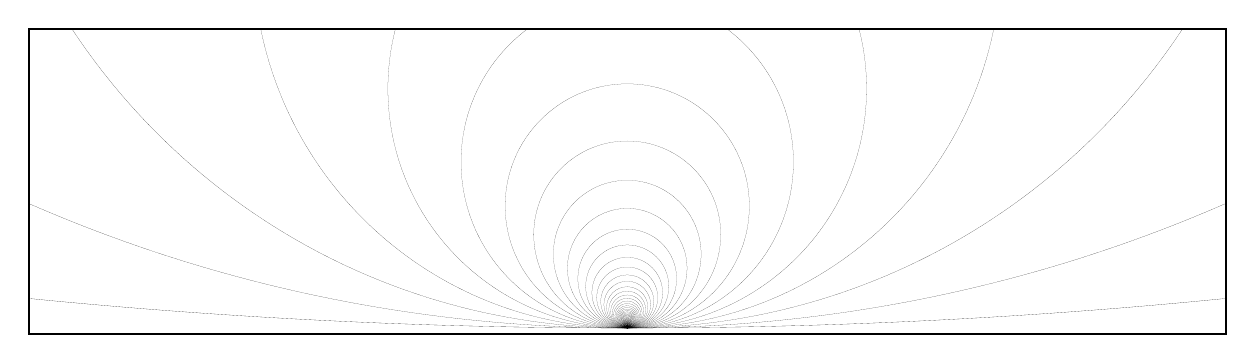
\begin{tikzpicture}[scale = 76]
	\draw[thick] (-.1,-.001) rectangle (.1,.05);
	\clip (-.1,0) rectangle (.1,.05); % remove for all circles
	\foreach \i in {1,...,100}{
		\draw[line width=0.1/\i mm] (0, 1/\i^2) circle (1/\i^2);
	}
	\end{tikzpicture}
	\caption{A closeup of the Hawaiian earring $\mathbb{H}^1$.}
	\label{fig:earrings}
\end{figure}

\begin{thm} \label{thm:counterexample}
	The function $f \colon \HE \to \R$ whose value at the origin is $0$ and is $1$ everywhere else defines a compact $\LC$ sublevel set filtration that is not q-tame with respect to $\H$ if $\H_{n}(\HE)$ is not finite dimensional for some $n$.
\end{thm}

\begin{proof}
	The space $\HE$ is Hausdorff and locally compact since $\R^{d+1}$ is.
	To verify that $f$ has compact sublevel sets we notice that all level sets are either the empty set, the singleton containing the origin, or $\HE$ itself, all compact spaces.
	Let us now verify that the sublevel set filtration of $f$ is weakly $\LC$.
	Let $\epsilon > 0$ and $x \in \HE$.
	If $x$ is the origin, we choose $\delta$ between $0$ and the minimum of $\epsilon$ and $1$.
	Then $\HE_{\leq f(x) + \delta} = \HE_{\leq \delta} = \{x\}$, so the weak $\LC$ condition is trivially satisfied.
	For $x$ not the origin, there is a unique $d$-sphere in $\HE$ that contains it.
	Clearly, we may choose $\delta > 0$ so small that $D_\delta(x) = \{y \in \R^{d+1} \mid \Vert x - y \Vert < \delta\} \cap \HE$ is a disk contained in this sphere, so $D_\delta(x)$ can be contracted to $\{x\}$ and the weak $\LC$ condition again follows trivially.
	What remains to be shown is that $\HE_{\leq \bullet}$ is not q-tame for $\H$.
This follows directly from our assumption that $\H_{n}(\HE)$ is not finite dimensional for some $n$ because $\HE_{\leq t}$ is constant with value $\HE$ for $t \geq 1$.
\end{proof}

Both singular and \v{C}ech homology of the Hawaiian earring are infinite dimensional in some degree, so they satisfy the assumptions of \cref{thm:counterexample}.
The singular case is treated in \cite{Barratt.1962}, and for \v{C}ech homology, one can use the fact that it commutes with totally ordered limits for compact Hausdorff spaces \cite[Theorems VIII.3.6.\@ and X.3.1.]{MR0050886}:
Define 
\begin{align*}
\HE_k &= \left\{ (x_0, \dots, x_d) \in \R^{d+1} \ \middle|\  \left( x_0 - \frac{1}{k} \right)^2 + x_1^2 + \dots + x_d^2 \leq \left( \frac{1}{k} \right)^2 \right\} \\
& \cup \bigcup_{n=1}^{k-1} \left\{ (x_0, \dots, x_d) \in \R^{d+1} \ \middle|\  \left( x_0 - \frac{1}{n} \right)^2 + x_1^2 + \dots + x_d^2 = \left( \frac{1}{n} \right)^2 \right \},
\end{align*}
i.e., the $d$-dimensional Hawaiian earring but with the $k$-th largest $d$-sphere filled.
We have $\lim_{k} \HE_{k} = \bigcap_{k} \HE_{k} = \HE$, and hence $\CH_{d}(\HE; \mathbb{F}) = \lim_{k} \CH_{d}(\HE_{k}; \mathbb{F})$, where $\CH$ denotes \v{C}ech homology.
Clearly, each $\HE_{k}$ is a CW-complex, so we can simply use cellular homology to compute
\begin{equation*}
\lim_{k}\CH_{d}(\mathbb{H}^{d}_{k}; \mathbb{F})=\lim\left(\dots\to \prod_{n=1}^2\mathbb{F}\to \prod_{n=1}^1\mathbb{F}\to \prod_{n=1}^0\mathbb{F}\right)=\prod_{n\in\mathbb{N}}\mathbb{F},
\end{equation*}
which is infinite-dimensional over $\mathbb{F}$.

\begin{cor}
    The function $f \colon \HE \to \R$ whose value at the origin is $0$ and is $1$ everywhere else defines a weakly $\LC$ compact sublevel set filtration that is not q-tame with respect to singular and \v{C}ech homology.
\end{cor}

The gap we have highlighted in the argument of Morse and Tompkins can be fixed by applying \cref{t:strong local connectedness implies q-tameness} because the proof given in \cite[p.464]{Morse.1939} for local connectivity of $(\Omega_g, A_g)$ actually establishes a stronger property for the sublevel set filtration of $A_g$, which we now formalize.

\begin{defi}
	The sublevel set filtration of a function $f \colon X \to \R$ is said to be \emph{strongly} $\LC$ if for any $x \in X$, any neighborhood $V$ of $x$ and any pair of indices $f(x) < s < t$ there is a neighborhood $U \subseteq V$ of $x$ such that the map $f_{\leq s} \cap U \to f_{\leq t} \cap V$ is homotopic to a constant map.
\end{defi}

Clearly, the filtration being strongly $\LC$ implies that the filtration is also strongly $\HLC$ for \v{C}ech homology with field coefficients, which is what Morse and Tompkins use.
Therefore, from \cref{t:strong local connectedness implies q-tameness} we can conclude that $(\Omega_g, A_g)$ is \mbox{q-tame} as claimed.
This implies that Morse inequalities hold, and hence so does the Morse-Tompkins' Unstable Minimal Surfaces Theorem.

We have also mentioned that Morse introduced another condition that he also called local $F$-connectivity three years earlier.
It roughly corresponds to being \emph{strongly} $\piLC$ with a certain added uniformity property.
In the original it reads:
\begin{displaycquote}[p.421-422]{Morse.1937}
	The space $M$ will be said to be locally $F$-connected for the order $n$ if corresponding to $n$, an arbitrary point $p$ on $M$, and an arbitrary positive constant $e$, there exists a positive constant $\delta$ with the following property.
For $c \geq F(p)$ any singular $n$-sphere on $F \leq c$ (the continuous image on $F \leq c$ of an ordinary $n$-sphere) on the $\delta$-neighborhood $p_{\delta}$ of $p$ is the boundary of a singular $(n + 1)$-cell on $F \leq c + e$ and on $p_e$.
\end{displaycquote}
Morse also claims in the given reference that this condition is sufficient for q-tameness, but without providing a proof.
We expect this statement to be true, but do not investigate it further.